\chapter{Tableaux et figures}
\label{chap:tableaux}

Les tableaux et graphiques ne sont pas les éléments de texte les plus
simples et rapides à créer avec {\LaTeX}. Les traitements de texte
brillent, ici, avec leurs interfaces graphiques permettant de composer
un tableau ou un graphique simple pièce par pièce avec la souris.

En revanche, pour ce type de contenu comme pour tout autre, {\LaTeX}
fait ce qu'on lui demande, sans tenter de deviner notre pensée ou,
pire, de prétendre savoir mieux que nous ce que nous voulons faire. À
ce chapitre, les traitements de texte ne brillent plus! Peut-être avez-vous
déjà eu de la difficulté à contrôler les bordures d'un tableau, la
hauteur des lignes ou la largeur des colonnes dans un traitement de
texte? Alors vous comprenez que l'exercice de composition d'un tableau
peut rapidement devenir frustrant.

Avant de discuter de la création ou de l'insertion de tableaux, de
graphiques et d'images dans un document {\LaTeX}, il convient de
présenter très succinctement quelques règles à suivre pour concevoir
des tableaux clairs et faciles à consulter.


\section{De la conception de beaux tableaux}
\label{sec:tableaux:booktabs}

On utilise les tableaux pour disposer de l'information sous forme de
grille. Par conséquent, le premier réflexe pour les mettre en forme
consiste souvent à mettre en évidence cette grille par le biais de
filets\footnote{%
  Terme typographique pour ce qui est communément appelés des «lignes»
  dans le langage courant ou des «bordures» dans les logiciels de
  traitement de texte. Dans la documentation en anglais, on parle de
  \emph{rules}.} %
horizontaux et verticaux.

C'est une mauvaise idée, une pratique à éviter. Vraiment!

Comparer les deux tableaux ci-dessous. Le premier est mis en forme
selon une approche classique supportée depuis toujours par {\LaTeX}:
filets doubles en entête et en pied de tableau, filets simples entre
chaque ligne et entre les colonnes.

\begin{center}
  \begin{tabular}{|>{$}c<{$}|>{$}r<{$}|>{$}r<{$}|>{$}r<{$}|>{$}c<{$}|>{$}c<{$}|}
    \hline\hline
    i &
    \multicolumn{1}{c|}{$v$} &
    \multicolumn{1}{c|}{$b_i$} &
    \lfloor v/b_i \rfloor & v \bmod b_i & x_i \\
    \hline
    0 & \nombre{91492} &  60 & \nombre{1524} & 52 & 52 \\
    1 &  \nombre{1524} &  60 &           25  & 24 & 24 \\
    2 &            25  &  24 &            1  &  1 &  1 \\
    3 &             1  & 365 &            0  &  1 &  1 \\
    \hline\hline
  \end{tabular}
\end{center}

Le second tableau tire profit des fonctionnalités du paquetage
\pkg{booktabs} et des recommandations de son auteur: les filets
horizontaux sont d'épaisseur différente selon qu'ils sont situés dans
l'entête et dans le pied du tableau ou entre les lignes, l'espace
autour des filets horizontaux est plus grand et, surtout, il n'y a pas
de filets verticaux.

\begin{center}
  \begin{tabular}{>{$}c<{$}>{$}r<{$}>{$}r<{$}>{$}r<{$}>{$}c<{$}>{$}c<{$}}
    \toprule
    i &
    \multicolumn{1}{c}{$v$} &
    \multicolumn{1}{c}{$b_i$} &
    \lfloor v/b_i \rfloor & v \bmod b_i & x_i \\
    \midrule
    0 & \nombre{91492} &  60 & \nombre{1524} & 52 & 52 \\
    1 &  \nombre{1524} &  60 &           25  & 24 & 24 \\
    2 &            25  &  24 &            1  &  1 &  1 \\
    3 &             1  & 365 &            0  &  1 &  1 \\
    \bottomrule
  \end{tabular}
\end{center}

La seconde version n'est-elle pas la plus aérée et la plus facile à
consulter? N'est-ce pas que, contrairement à ce que l'on pourrait
penser, les filets verticaux ne sont pas du tout requis pour bien
délimiter les colonnes?

Tel que mentionné ci-dessus, le paquetage \pkg{booktabs} ajoute des
fonctionnalités à {\LaTeX} pour améliorer la qualité typographique des
tableaux. Dans la documentation du paquetage, son auteur énonce
quelques règles à suivre pour la mise en forme des tableaux:
\begin{enumerate}
\item ne \emph{jamais} utiliser de filets verticaux. Si l'information
  du côté gauche du tableau semble si différente de celle du côté
  droit qu'un filet vertical apparaît absolument nécessaire, scinder
  simplement l'information dans deux tableaux;
\item ne jamais utiliser de filets doubles;
\item placer les unités (\$, cm, {\textdegree}C, etc.) dans le titre
  de la colonne plutôt qu'après chaque valeur dans le corps du
  tableau;
\item toujours inscrire un chiffre du côté gauche du séparateur
  décimal: $0,1$ et non $,1$ (pratique plus répandue en anglais, où le
  séparateur décimal est le point);
\item ne pas utiliser un symbole pour représenter une valeur
  répétée (comme $''$ ou ---). Laisser un blanc ou répéter la
  valeur s'il subsiste une ambiguïté.
\end{enumerate}

Nous recommandons évidemment de suivre ces règles et c'est pourquoi la
présente documentation ainsi que les fichiers d'exemples font usage
des commandes de \pkg{booktabs}.

Les fonctionnalités de \pkg{booktabs} sont intégrées à la classe
\class{memoir} et par conséquent à \class{ulthese}. Il n'est donc pas
nécessaire de charger le paquetage avec ces deux classes.



\section{Tableaux}
\label{sec:tableaux:tableaux}

Peu importe l'outil informatique utilisé, la création d'un tableau
requiert toujours de préciser à l'ordinateur le nombre de colonnes que
contiendra le tableau, l'entête du tableau le cas échéant et le contenu
des différentes cellules. Cette dernière étape nécessite à son tour
une convention pour indiquer les passages à la colonne suivante
ainsi que le passage à la ligne suivante.

On crée des tableaux dans {\LaTeX} principalement avec les
environnements \Ie{tabular}, \Ie{tabular*} et \Ie{tabularx} (ce
dernier fourni par le paquetage \pkg{tabularx} ou par la classe
\class{memoir}). La syntaxe de ces environnements est:
\begin{lstlisting}
\begin{tabular}`\marg{format}'           `\textit{lignes}' \end{tabular}
\begin{tabular*}`\marg{largeur}\marg{format}' `\textit{lignes}' \end{tabular*}
\begin{tabularx}`\marg{largeur}\marg{format}' `\textit{lignes}' \end{tabularx}
\end{lstlisting}
La signification des arguments\footnote{%
  Nous avons omis un argument optionnel à peu près jamais utilisé
  servant à spécifier l'alignement vertical du tableau par rapport à
  la ligne de base externe.} %
est la suivante. Nous ne traitons ici que les options les plus souvent
employées. Pour une liste plus exhaustive, consulter la documentation
de la classe \class{memoir} (chapitre 11) ou %
\citet[section \link{http://fr.wikibooks.org/wiki/LaTeX/Tableaux}{Tableaux}]{wikilivres:latex}.

\begin{list}{}{%
    \setlength{\labelsep}{1.5ex}
    \settowidth{\labelwidth}{\meta{largeur}}
    \setlength{\leftmargin}{\labelwidth}
    \addtolength{\leftmargin}{\labelsep}
    \setlength{\parsep}{0.5ex plus0.2ex minus0.2ex}
    \setlength{\itemsep}{0.3ex}
    \renewcommand{\makelabel}[1]{\meta{#1}\hfill}}
%
\item[largeur] Largeur hors tout d'un tableau avec les
  environnements \Pe{tabular*} et \Pe{tabularx}. Autrement,
  avec l'environnement \Pe{tabular}, la largeur d'un tableau est
  déterminée automatiquement pour contenir tout le contenu du tableau,
  quitte à dépasser dans la marge de droite.

  La largeur du tableau est généralement exprimée en fraction de la
  largeur du bloc de texte. Celle-ci est accessible avec la commande
  \cs{textwidth}. Par exemple, les déclarations suivantes
  définissent respectivement des tableaux occupant toute la largeur
  d'une page et 80~\% de la largeur de la page:
\begin{lstlisting}
\begin{tabular*}{\textwidth}`\marg{format}'
\end{lstlisting}
\begin{lstlisting}
\begin{tabularx}{0.8\textwidth}`\marg{format}'
\end{lstlisting}
  L'environnement \Ie{tabular*} joue sur l'espace entre les colonnes
  pour parvenir à la largeur prescrite, alors que \Ie{tabularx} joue
  sur la largeur des colonnes (voir ci-dessous).
  %
\item[format] Le format des colonnes et, par le fait même, le nombre
  de colonnes puisque l'argument doit compter un symbole pour chaque
  colonne du tableau. Les principaux symboles de mise en forme des
  colonnes sont:
  \begin{description}
  \item[\normalfont\code{l}] contenu de la colonne aligné à gauche;
  \item[\normalfont\code{r}] contenu de la colonne aligné à droite;
  \item[\normalfont\code{c}] contenu de la colonne centré;
  \item[\normalfont\code{p\{}\textit{lgr}\code{\}}] contenu de la colonne traité comme un
    paragraphe de texte de largeur \textit{lgr};
  \item[\normalfont\code{X}] [environnement \Ie{tabularx} seulement]
    colonne dont la largeur peut être ajustée pour obtenir un tableau
    de la largeur prescrite; identique à \code{p} par ailleurs.
  \end{description}
  Par exemple, pour définir un tableau à trois colonnes dont le
  contenu de la première est aligné à gauche, celui de la seconde à
  droite et celui de la troisième en texte libre dans une cellule de
  5~cm de largeur, on utiliserait:
\begin{lstlisting}
\begin{tabular}{lrp{5cm}}
\end{lstlisting}
  Avec la déclaration suivante, la largeur de la troisième colonne
  sera automatiquement adaptée pour que le tableau occupe toute la
  largeur de la page:
\begin{lstlisting}
\begin{tabularx}{\textwidth}{lrX}
\end{lstlisting}

  Les symboles \verb=|= et \verb=||= dans \textit{format} servent à
  insérer des filets verticaux simples et doubles entre les colonnes,
  mais nous avons vu à la \autoref{sec:tableaux:booktabs} que c'est
  une pratique à proscrire.
  %
\item[lignes] Le contenu des cellules du tableau. Les entrées des
  cellules sont séparées par le symbole \verb=&= et les lignes par
  \verb=\\=. Une cellule peut être vide.

  Les lignes de contenu peuvent également contenir certaines commandes
  spéciales pour contrôler la mise en forme. La commande ci-dessous
  permet de fusionner des cellules:
  \begin{description}
  \item[\normalfont\cmd{\multicolumn\marg{num}\marg{fmt}\marg{texte}}]
    fusionne les \meta{num} cellules suivantes en une seule de format
    \meta{fmt} et contenant le texte \meta{texte}. \par%
    Cette commande ne peut apparaître qu'au début d'une ligne ou après
    un symbole de changement de colonne \verb=&=. \par%
    La commande est souvent utilisée avec une valeur de
    $\text{\meta{num}}$ égale à 1 pour changer le format d'une
    cellule, par exemple pour centrer le titre d'une colonne autrement
    alignée à gauche ou à droite.
  \end{description}

  Les commandes suivantes\footnote{%
    Ce sont les commandes de \pkg{booktabs} et \class{memoir}
auxquelles nous faisions référence à la \autoref{sec:tableaux:booktabs}.} %
  servent à insérer des filets horizontaux dans un tableau:
  \begin{description}
  \item[\normalfont\cmd{\toprule}] insère un filet horizontal épais
    suivi d'un espace vertical au début d'un tableau;
  \item[\normalfont\cmd{\midrule}] insère un filet horizontal mince
    précédé et suivi d'un espace vertical entre deux lignes;
  \item[\normalfont\cmd{\cmidrule\marg{n-m}}] insère un filet
    horizontal comme \cmd{\midrule}, mais seulement de la gauche de la
    colonne \meta{n} à la droite de la colonne \meta{m};
  \item[\normalfont\cmd{\bottomrule}] insère un filet horizontal épais
    précédé d'un espace vertical à la fin d'un tableau.
  \end{description}
  Une fin de ligne \verb=\\=  doit  obligatoirement précéder chacune
  de ces commandes, sauf évidemment \cmd{\toprule}.

  Un exemple simple de lignes de contenu serait:
\begin{lstlisting}
\toprule
Produit & Quantité & Prix unitaire (\$) & Prix (\$) \\
\midrule
Vis à bois    & 2 & 9,90 & 19,80 \\
Clous vrillés & 5 & 4,35 & 21,75 \\
\midrule
TOTAL         & 7 &      & 41,55 \\
\bottomrule
\end{lstlisting}
\end{list}

La hauteur des lignes d'un tableau est déterminée automatiquement en
fonction du contenu de celles-ci.

\begin{exemple}
  \label{exemple:tableaux:tabular}
  On reprend le contenu ci-dessus pour en faire un tableau d'une
  largeur ajustée automatiquement au contenu. La première colonne est
  alignée à gauche et toutes les autres à droite.
\begin{lstlisting}
\begin{tabular}{lrrr}
  \toprule
  Produit & Quantité & Prix unitaire (\$) & Prix (\$) \\
  \midrule
  Vis à bois    & 2 & 9,90 & 19,80 \\
  Clous vrillés & 5 & 4,35 & 21,75 \\
  \midrule
  TOTAL         & 7 &      & 41,55 \\
  \bottomrule
\end{tabular}
\end{lstlisting}
  \begin{center}
    \begin{tabular}{lrrr}
      \toprule
      Produit & Quantité & Prix unitaire (\$) & Prix (\$) \\
      \midrule
      Vis à bois    & 2 & 9,90 & 19,80 \\
      Clous vrillés & 5 & 4,35 & 21,75 \\
      \midrule
      TOTAL         & 7 &      & 41,55 \\
      \bottomrule
    \end{tabular}
  \end{center}

  Avec quelques modifications, le tableau occupe maintenant toute la
  largeur de la page, la largeur de la première colonne étant ajustée
  pour combler l'espace nécessaire. De plus, on modifie l'entête de la
  première colonne avec la commande \cmd{\multicolumn} afin de centrer
  le titre. Enfin, on augmente la hauteur de l'entête à l'aide d'une
  réglure invisible (\autoref{sec:boites:rulebox}).
\begin{lstlisting}
\begin{tabularx}{\textwidth}{Xrrr}
  \toprule
  \multicolumn{1}{c}{Produit} &
    \rule[-8pt]{0mm}{24pt} Quantité &
    Prix unitaire (\$) & Prix (\$) \\
  \midrule
  Vis à bois    & 2 & 9,90 & 19,80 \\
  Clous vrillés & 5 & 4,35 & 21,75 \\
  \midrule
  TOTAL         & 7 &      & 41,55 \\
  \bottomrule
\end{tabularx}
\end{lstlisting}
  \begin{center}
    \begin{tabularx}{\textwidth}{Xrrr}
      \toprule
      \multicolumn{1}{c}{Produit} &
      \rule[-8pt]{0mm}{24pt} Quantité & Prix unitaire (\$) & Prix (\$) \\
      \midrule
      Vis à bois    & 2 & 9,90 & 19,80 \\
      Clous vrillés & 5 & 4,35 & 21,75 \\
      \midrule
      TOTAL         & 7 &      & 41,55 \\
      \bottomrule
    \end{tabularx}
  \end{center}
  \qed
\end{exemple}



\section{Figures et graphiques}
\label{sec:tableaux:figures}

Il est possible de tracer des figures simples directement avec {\LaTeX}. Par «simple» on entend: des figures se
limitant  pour l'essentiel à du texte, des lignes, des flèches, des
ronds et des ovales. C'est parfois amplement suffisant et, en
définitive, assez pratique puisque le code source d'une figure se
trouve alors dans le même format que le reste du document.

Pour la création de figures et de graphiques plus complexes, on aura généralement
recours à des logiciels spécialisés externes. {\LaTeX} est ensuite en
mesure d'importer des graphiques dans les formats standards tels que PDF, JPEG
ou PNG, voire même d'insérer dans un document une ou plusieurs pages
d'un document PDF.

Couvrir les détails de la création et de la manipulation d'images
dépasse largement la portée du présent document. Le reste de cette
section ne présente que les principales fonctionnalités. Le lecteur
intéressé d'en savoir plus pourra se référer aux sources de documentation habituelles figurant à la
bibliographie.


\subsection{Figures {\LaTeX}}
\label{sec:tableaux:figures:picture}

L'environnement \Ie{picture} permet de tracer des figures simples dans
{\LaTeX} comme des diagrammes à base de texte, des flux logiques ou
des organigrammes. Quelques logiciels spécialisés de création de
graphiques sont en mesure d'exporter leurs graphiques dans le format
de \Ie{picture}.

Une fois conçues, les figures réalisées avec \Pe{picture} sont
simples à modifier; nul besoin de recourir à un logiciel externe pour
le moindre petit changement. Autre avantage: la police de caractère du texte
de la figure sera le même que celle du document.

Pour tracer une figure avec l'environnement \Pe{picture}, on crée
d'abord une grille (invisible) d'une dimension quelconque dans l'unité
de mesure de son choix (autrement dit: les lignes de la grille
peuvent être distantes aussi bien de \code{1pt} que de \code{1cm}).
Ensuite, on dispose des éléments sur la grille en donnant les
coordonnées du point d'ancrage et, le cas échéant, les dimensions de
l'élément, la distance à parcourir ou quelqu'autre information pour
compléter l'élément. C'est souvent plus simple d'esquisser d'abord un modèle au
crayon sur du papier quadrillé.

La figure ci-dessous illustre ce qu'il est possible de faire avec
l'environnement \Pe{picture}. La consultation du code commenté correspondant devrait
permettre de comprendre les principes de base de la création de
figures. Autrement, l'annexe~D de la %
 \doc{memman}{http://texdoc.net/pkg/memoir} %
de la classe \class{memoir} fournit une bonne introduction à \Pe{picture}.

(Nous avons tracé la grille en filigrane dans la figure afin de
faciliter la comparaison entre le code et le résultat.)

\setlength{\unitlength}{7mm}
\begin{center}
  \begin{picture}(15,9)
    \linethickness{0.3pt} \color{lightgray}
    \multiput(0,0)(1,0){16}{\line(0,1){9}}
    \multiput(0,0)(0,1){10}{\line(1,0){15}}
    \color{black}

    %% boîtes
    \put(0,7){%
      \framebox(5,1.5){
        \begin{minipage}{35mm}
          \centering L'environnement \\ \texttt{picture}
        \end{minipage}}}

    \put(1,4.5){\circle{2}}
    \put(1,4.5){\makebox(0,0){\small convient}}
    \put(4,3){\circle{2}}
    \put(4,3){\makebox(0,0){\small bien}}

    \put(8.5,5.7){pour les diagrammes}

    \thicklines
    \put(8,1){\dashbox{0.2}(7,1.5){et autres figures simples.}}

    %% lignes
    \thinlines
    \put(1,7){\vector(0,-1){1.5}}

    \put(14,5.75){\circle*{0.1}}
    \put(14,5.75){\vector(-1,-1){3.25}}

    \thicklines
    \put(1,3.5){\line(0,-1){0.5}}
    \put(1,3){\vector(1,0){2}}

    \qbezier(4,2)(5.5,-0.5)(7,4.25)
    \qbezier(7,4.25)(8.5,9)(10,6.5)
    \put(10,6.5){\vector(2,-3){0}}
  \end{picture}
\end{center}

\begingroup
  \small
\begin{lstlisting}
\setlength{\unitlength}{7mm}  % unité de mesure
\begin{picture}(15,9)         % grille 15 x 9
  %%%
  %%% On trace d'abord toutes les boîtes
  %%%
  %% Rectangle "L'environnement picture"
  \put(0,7){%                 % point d'ancrage (0, 7)
    \framebox(5,1.5){%        % rectangle 5 x 1,5 plein
      \begin{minipage}{35mm}  % contenu de la boîte
        \centering L'environnement \\ \texttt{picture}
      \end{minipage}}}

  %% Cercles "convient" et "bien"
  \put(1,4.5){\circle{2}}                     % cercle de diamètre 2
  \put(1,4.5){\makebox(0,0){\small convient}} % texte centré
  \put(4,3){\circle{2}}                       % autre cercle
  \put(4,3){\makebox(0,0){\small bien}}       % texte

  %% Texte "pour les diagrammes"
  \put(8.5,5.7){pour les diagrammes} % point d'ancrage (8,5, 5,7)

  %% Rectangle pointillé "et autres figures simples."
  \thicklines                     % lignes grasses
  \put(8,1){\dashbox{0.2}(7,1.5){ % rectangle 7 x 1,5 pointillé
      et autres figures simples.}}

  %%%
  %%% On trace ensuite les lignes entre les boîtes
  %%%
  %% De "L'environnement picture" à "convient"
  \thinlines                    % retour aux lignes minces
  \put(1,7){\vector(0,-1){1.5}} % flèche vers le bas de longueur 1,5
                                % [couple (0,-1) donne la pente]

  %% De "pour les diagrammes" à "et autres figures simples."
  \put(14,5.75){\circle*{0.1}}  % petit cercle plein
  \put(14,5.75){\vector(-1,-1){3.25}} % flèche vers sud-ouest
                                      % [3.25 est déplacement hor.]

  %% Entre les deux cercles; requiert deux segments
  \thicklines                   % lignes grasses
  \put(1,3.5){\line(0,-1){0.5}} % courte ligne vert. sans flèche
  \put(1,3){\vector(1,0){2}}    % flèche horizontale

  %% Entre "bien" et "pour les diagrammes"; requiert deux courbes
  \qbezier(4,2)(5.5,-0.5)(7,4.25)  % deux courbes de Bézier bout à
  \qbezier(7,4.25)(8.5,9)(10,6.5)  % bout pour produire courbe en S
  \put(10,6.5){\vector(2,-3){0}}   % pointe de flèche seule
\end{picture}
\end{lstlisting}
\endgroup


Il existe quelques outils pour tracer des figures plus complexes
directement avec {\TeX}, dont PSTricks \citep{pstricks}
ou le système Ti\emph{k}Z/\textsc{pgf} \citep{tikz}.
Ce dernier gagne beaucoup en popularité depuis quelques années.


\subsection{Importation d'images}
\label{sec:tableaux:figures:graphics}

Il est aujourd'hui simple d'importer des images de source externes
dans un document {\LaTeX} en utilisant l'un ou l'autre des paquetages
\pkg{graphics} ou \pkg{graphicx} \citep{graphicx} en combinaison avec
un moteur {\TeX} moderne tel que pdf{\LaTeX} ou {\XeLaTeX}. Les
fonctionnalités des deux paquetages sont les mêmes, seules les
syntaxes des commandes diffèrent. Nous présenterons les commandes de
\pkg{graphicx}, plus modernes et conviviales.

La commande de base pour importer des images dans un document {\LaTeX} est
\begin{lstlisting}
\includegraphics`\oarg{options}\marg{fichier}'
\end{lstlisting}
où \meta{fichier} est le nom du fichier à importer. Il n'est pas
nécessaire de préciser l'extension dans le nom de fichier pour les
types d'images usuelles. Avec les moteurs pdf{\LaTeX} et {\XeLaTeX},
les types d'images automatiquement reconnus sont au moins PDF, JPEG et
EPS.

Les \meta{options} de \cmd{\includegraphics}, nombreuses, permettent
de redimensionner une image, de la faire pivoter ou encore de n'en
importer qu'une partie. L'exemple ci-dessous présente les principales
fonctionnalités; consulter la %
\doc{grfguide}{http://texdoc.net/pkg/graphics/} %
pour les détails et d'autres options.

\begin{exemple}
  Le fichier \fichier{ul\_p.pdf} contenant le logo de l'Université
  Laval en couleur et en format vectoriel est distribué avec la
  présente documentation ainsi qu'avec la classe \class{ulthese}. La
  simple commande
\begin{lstlisting}

\includegraphics{ul_p}
\end{lstlisting}
  insère le fichier en pleine grandeur dans le document:
  \begin{trivlist}
  \item 
\includegraphics{ul_p}
  \end{trivlist}

  On peut redimensionner l'image en valeur relative avec l'option
  \code{scale} ou en valeur absolue avec les options \code{width} ou
  \code{height}:
  \begin{trivlist}
  \item %
    \begin{minipage}[t]{0.62\linewidth}
\begin{lstlisting}
%% réduction à 40 % de taille réelle

\includegraphics[scale=0.4]{ul_p}
\end{lstlisting}
    \end{minipage}
    \hfill
    \begin{minipage}[t]{0.35\linewidth}
      \mbox{}\\ 
\includegraphics[scale=0.4]{ul_p}
    \end{minipage}
  \item %
    \begin{minipage}[t]{0.62\linewidth}
\begin{lstlisting}
%% réduction à 15 mm de haut

\includegraphics[height=15mm]{ul_p}
\end{lstlisting}
    \end{minipage}
    \hfill
    \begin{minipage}[t]{0.35\linewidth}
      \mbox{}\\ 
\includegraphics[height=15mm]{ul_p}
    \end{minipage}
  \end{trivlist}
  (Il est préférable d'utiliser une seule de \code{width} ou
  \code{height}. Autrement, ajouter l'option
  \verb|keepaspectratio=true| pour éviter de déformer l'image.)

  L'option \code{angle} permet de faire pivoter l'image dans le sens
  inverse des aiguilles d'une montre autour du coin inférieur gauche
  de l'image:
  \begin{trivlist}
  \item %
    \begin{minipage}[t]{0.7\linewidth}
\begin{lstlisting}
%% réduction à 25 % et rotation à 45 degrés

\includegraphics[angle=45,scale=0.25]{ul_p}
\end{lstlisting}
    \end{minipage}
    \hfill
    \begin{minipage}[t]{0.25\linewidth}
      \mbox{}\\ 
\includegraphics[angle=45,scale=0.25]{ul_p}
    \end{minipage}
  \end{trivlist}

  Enfin, il y a diverses manières de sélectionner une partie seulement
  d'une image. L'option \code{bb} (pour \emph{Bounding Box}) prend
  quatre mesures en points PostScript (\code{bp}; $1~\text{bp} =
  1/72~\text{pouce}$) définissant le coin inférieur gauche et le coin
  supérieur droit de la zone à inclure:
  \begin{trivlist}
  \item %
    \begin{minipage}[t]{0.7\linewidth}
\begin{lstlisting}
%% extraction du logo seul et réduction

\includegraphics[bb=0 0 102 129,clip=true,
  scale=0.4]{ul_p}
\end{lstlisting}
    \end{minipage}
    \hfill
    \begin{minipage}[t]{0.25\linewidth}
      \mbox{}\\ 
\includegraphics[bb=0 0 102 129, clip=true, scale=0.4]{ul_p}
    \end{minipage}
  \end{trivlist}
  \qed
\end{exemple}

La commande \cmd{\includegraphics} permet d'appliquer certaines
 transformations aux images importées, mais celles-ci
peuvent également s'effectuer à l'aide de commandes externes
\emph{après} l'importation. L'avantage de ces commandes, c'est
qu'elles sont valides tout autant pour du texte que pour des images.

Le paquetage \pkg{graphicx} définit les commandes suivantes:
\begin{lstlisting}
\rotatebox`\oarg{options}\marg{angle}\marg{texte}'
\scalebox`\marg{échelle-h}\oarg{échelle-v}\marg{texte}'
\resizebox`\marg{dim-h}\marg{dim-v}\marg{texte}'
\reflectbox`\marg{texte}'
\end{lstlisting}
Dans tous les cas, \meta{texte} peut être du simple texte ou une boîte
quelconque, y compris le résultat de \cmd{\includegraphics}. Ainsi,
\begin{lstlisting}
\rotatebox{45}{
\includegraphics{ul_p}}
\end{lstlisting}
et
\begin{lstlisting}

\includegraphics[angle=45]{ul_p}
\end{lstlisting}
donnent le même résultat.

Avec \cmd{\scalebox}, la mise à l'échelle \meta{échelle-h} s'applique
par défaut autant à l'horizontale qu'à la verticale. Autrement,
\meta{texte} est déformé.  Avec \cmd{\resizebox}, on peut spécifier
l'une de \meta{dim-h} ou \meta{dim-v} et \verb=!= pour l'autre valeur
pour éviter de déformer \meta{texte}.

\begin{exemple}
  Voici des exemples d'utilisation des commandes \cmd{\rotatebox},
  \cmd{\scalebox}, \cmd{\resizebox} et \cmd{\reflectbox} avec du texte:
  \begin{trivlist}
  \item %
    \begin{minipage}{0.55\linewidth}
\begin{lstlisting}
\rotatebox{135}{texte}
\end{lstlisting}
    \end{minipage}
    \hfill
    \begin{minipage}{0.35\linewidth}
      \rotatebox{135}{texte}
    \end{minipage}
  \item %
    \begin{minipage}{0.55\linewidth}
\begin{lstlisting}
\scalebox{1.5}{texte}
\end{lstlisting}
    \end{minipage}
    \hfill
    \begin{minipage}{0.35\linewidth}
      \scalebox{1.5}{texte}
    \end{minipage}
  \item %
    \begin{minipage}{0.55\linewidth}
\begin{lstlisting}
\scalebox{1.5}[0.75]{texte}
\end{lstlisting}
    \end{minipage}
    \hfill
    \begin{minipage}{0.35\linewidth}
      \scalebox{1.5}[0.75]{texte}
    \end{minipage}
  \item %
    \begin{minipage}{0.55\linewidth}
\begin{lstlisting}
\resizebox{3cm}{!}{texte}
\end{lstlisting}
    \end{minipage}
    \hfill
    \begin{minipage}{0.35\linewidth}
      \resizebox{3cm}{!}{texte}
    \end{minipage}
  \item %
    \begin{minipage}{0.55\linewidth}
\begin{lstlisting}
\reflectbox{texte}
\end{lstlisting}
    \end{minipage}
    \hfill
    \begin{minipage}{0.35\linewidth}
      \reflectbox{texte}
    \end{minipage}
  \end{trivlist}
  \qed
\end{exemple}



\subsection{Insertion de documents PDF}
\label{sec:tableaux:figures:pdfpages}

Il est parfois utile d'insérer dans un document {\LaTeX} une ou
plusieurs pages d'un autre document en format PDF, et ce, sans avoir à
se soucier des marges respectives des deux documents. Si l'on utilise
les moteurs pdf{\LaTeX} ou {\XeLaTeX}, le très pratique paquetage
\pkg{pdfpages} \citep{pdfpages} fournit la commande
\begin{lstlisting}
\includepdf`\oarg{options}\marg{fichier}'
\end{lstlisting}
Les \meta{options} sont trop nombreuses pour les présenter ici;
consulter la %
\doc{pdfpages}{http://texdoc.net/pkg/pdfpages/}.

\begin{exemple}
  Les couvertures avant et arrière du présent document ont été
  réalisées dans un logiciel spécialisé de création graphique,
  sauvegardées dans un fichier \fichier{couvertures.pdf}, puis mises
  en place dans le document avec
\begin{lstlisting}

\includepdf[pages=1]{couvertures}

\includepdf[pages=2]{couvertures}
\end{lstlisting}
  aux endroits appropriés.
  \qed
\end{exemple}



\section{Éléments flottants}
\label{sec:tableaux:floats}

Dans la terminologie de {\LaTeX}, un élément flottant\footnote{%
  \emph{Float} en anglais.} %
est un bloc de contenu (une boîte, en fait) que le logiciel pourra
positionner sur la page et dans le document plus ou moins
automatiquement en fonction d'un algorithme prédéfini. C'est une
fonctionnalité très évoluée de {\LaTeX}.

Pourquoi voudrait-on laisser {\LaTeX} décider où un élément de contenu
devrait se retrouver dans notre document? D'abord et avant tout pour
les tableaux et les figures.

En effet, les tableaux et les figures sont des éléments de contenu qui occupent
souvent beaucoup d'espace vertical dans la page. S'il ne reste plus
assez de place pour y afficher un tel élément, {\LaTeX} devra
le déplacer au début de la page suivante et cela risque de produire une
page inesthétique car insuffisamment remplie\footnote{%
  \emph{Underful \cs{vbox}} dans le jargon de {\TeX}.}. %
Les traitements de texte génèrent sans rechigner des pages
à demi remplies dans de telles situations.

En définissant un élément comme flottant, on laisse plutôt à
{\LaTeX} la possibilité de le disposer au meilleur endroit en fonction
de la taille de l'élément, du contenu du document et de diverses
règles typographiques.

On crée des éléments flottants avec les environnements \Ie{table}
et \Ie{figure}:
\begin{lstlisting}
\begin{table}`\oarg{pos}'  `\textit{tableau}' \end{table}
\begin{figure}`\oarg{pos}' `\textit{figure}' \end{figure}
\end{lstlisting}
Ci-dessus, \meta{tableau} et \meta{figure} représentent le code source
d'un tableau ou d'une figure avec possiblement une commande
\cmd{caption}, tel que traité plus loin.

L'argument optionnel \meta{pos} permet d'indiquer à {\LaTeX}
la ou les positions \emph{souhaitées} pour le tableau ou la figure dans la page.
Lorsqu'il est question d'éléments flottants, il est très difficile de donner des
ordres fermes à {\LaTeX} et l'effet de l'argument \meta{pos} est
souvent déconcertant. Aussi vaut-il souvent mieux ne rien indiquer et
laisser {\LaTeX} faire à sa guise. Le résultat demeure assez
prévisible puisque {\LaTeX} tâchera d'insérer l'élément flottant dans
le document \emph{dès que possible} sous réserve des conditions
suivantes:
\begin{itemize}
\item l'élément flottant ne peut apparaître dans le document avant la
  page où l'élément est défini;
\item l'élément sera placé de préférence dans le haut de la page
  courante, puis dans le bas et enfin sur une page séparée ne pouvant
  contenir que des éléments flottants, mais pas de texte.
\end{itemize}

Si la décision de {\LaTeX} ne convient pas, il est possible de
l'infléchir avec une combinaison d'une ou plusieurs des lettres
suivantes dans l'argument \meta{pos};
\begin{description}
\item[\normalfont\code{b}] placer l'élément au bas (\emph{bottom}) de la page;
\item[\normalfont\code{h}] placer l'élément ici (\emph{here}), à
  l'endroit où il est défini dans le code source;
\item[\normalfont\code{p}] placer l'élément sur une page séparée;
\item[\normalfont\code{t}] placer l'élément au haut (\emph{top}) de la page;
\item[\normalfont\code{!}] essayer plus fort de placer l'élément à
  l'endroit spécifié dans le reste de l'argument.
\end{description}
La valeur par défaut de l'argument \meta{pos} est \code{tbp}. La
section~10.4 de la %
\doc{memman}{http://texdoc.net/pkg/memoir/} %
de \class{memoir} explique plus en détail la signification des valeurs
ci-dessus. Le lecteur qui voudrait vraiment \emph{tout} savoir sur la
disposition des éléments flottants pourra consulter
\cite{Mittelbach:floats:2014}.

\begin{exemple}
  On reprend le tableau de l'\autoref{exemple:tableaux:tabular}, mais cette
  fois défini à l'intérieur d'un environnement \Pe{table}:
\begin{lstlisting}
\begin{table}
  \centering
  \begin{tabular}{lrrr}
    \toprule
    Produit & Quantité & Prix unitaire (\$) & Prix (\$) \\
    \midrule
    Vis à bois    & 2 & 9,90 & 19,80 \\
    Clous vrillés & 5 & 4,35 & 21,75 \\
    \midrule
    TOTAL         & 7 &      & 41,55 \\
    \bottomrule
  \end{tabular}
\end{table}
\end{lstlisting}
  \begin{table}
    \centering
    \begin{tabular}{lrrr}
      \toprule
      Produit & Quantité & Prix unitaire (\$) & Prix (\$) \\
      \midrule
      Vis à bois    & 2 & 9,90 & 19,80 \\
      Clous vrillés & 5 & 4,35 & 21,75 \\
      \midrule
      TOTAL         & 7 &      & 41,55 \\
      \bottomrule
    \end{tabular}
  \end{table}
  Remarquer où {\LaTeX} a automatiquement placé le tableau dans le
  document en fonction des règles précitées. %
  \qed
\end{exemple}

Dans un document soigné, tout tableau et toute figure devrait
comporter une légende ainsi qu'un numéro afin de pouvoir les
annoncer et y faire référence dans le texte («comme l'illustre la
figure~3\dots»). Cela
permet à la fois de guider le lecteur au fil de sa lecture et de
construire une liste des tableaux et des figures\footnote{%
  Obtenues respectivement avec \cmd{\listoftables} et
\cmd{\listoffigures} \citep[section~3]{UL:latex:1}.} %
dans les pages liminaires d'un long document.

Pour ajouter une légende à un tableau ou une figure, il suffit
d'utiliser à l'intérieur des environnements \Ie{table} et \Ie{figure}
la commande
\begin{lstlisting}
\caption`\oarg{texte\_court}\marg{texte}'
\end{lstlisting}
où \meta{texte} est le texte de la légende. Si celui-ci est long
(plus d'une ligne), on peut en fournir une version abrégée dans
l'argument optionnel \meta{texte\_court}. C'est cette version abrégée
qui sera utilisée dans la liste des tableaux ou dans la liste des
figures.

La commande \cmd{\caption} insère,  à l'endroit où elle
apparait dans l'environnement, une légende de la forme «\textsc{Table}
\emph{n}~--~\meta{texte}» pour un tableau ou «\textsc{Figure}
\emph{n}~--~\meta{texte}» pour une figure. Le texte de la légende est
centré sur la page lorsqu'il fait moins d'une ligne; dans le cas
contraire il est disposé comme un paragraphe normal.

\begin{conseil}
  Les anciennes version du style français de \pkg{babel} utilisaient
  les étiquettes plus neutres «\textsc{Tab.}» et «\textsc{Fig.}» dans
  les légendes des tableaux et figures. Pour utiliser ces versions
  plutôt que les versions par défaut --- comme dans le présent
  document --- ajouter dans le préambule les commandes suivantes:
\begin{lstlisting}
\def\frenchtablename{{\scshape Tab.}}
\def\frenchfigurename{{\scshape Fig.}}
\end{lstlisting}
\end{conseil}

Pour faire référence à un tableau ou à une figure dans le texte, il
faut utiliser le système de renvois automatiques de {\LaTeX}
\citep[section~4]{UL:latex:1}. On attribue une étiquette à l'élément
flottant en plaçant la commande \cmd{\label} dans le texte de la
commande \cmd{\caption} ou dans son voisinage immédiat. Les commandes
\cmd{\ref} ou \cmd{\autoref} servent ensuite à insérer des renvois dans
le texte.

L'exemple suivant présente finalement la recette complète pour composer
un tableau et une figure dans {\LaTeX}, légende et renvoi inclus.

\begin{exemple}
  Attention, exemple récursif: son texte constitue lui-même un
  exemple. Le code source de la \autoref{fig:tableaux:captions} crée
  le \autoref{tab:tableaux:captions}.
  \begin{figure}
\begin{lstlisting}
\begin{table}
  \centering
  \caption{Tableau correspondant au code
    de la \autoref{fig:[...]}}
  \label{tab:[...]}
  \begin{tabular}{lrrr}
    \toprule
    Produit & Quantité & Prix unitaire (\$) & Prix (\$) \\
    \midrule
    Vis à bois    & 2 & 9,90 & 19,80 \\
    Clous vrillés & 5 & 4,35 & 21,75 \\
    \midrule
    TOTAL         & 7 &      & 41,55 \\
    \bottomrule
  \end{tabular}
\end{table}
\end{lstlisting}
    \caption{Code source pour créer le \autoref{tab:tableaux:captions}}
    \label{fig:tableaux:captions}
  \end{figure}
  \begin{table}
    \centering
    \caption{Tableau correspondant au code de la \autoref{fig:tableaux:captions}}
    \label{tab:tableaux:captions}
    \begin{tabular}{lrrr}
      \toprule
      Produit & Quantité & Prix unitaire (\$) & Prix (\$) \\
      \midrule
      Vis à bois    & 2 & 9,90 & 19,80 \\
      Clous vrillés & 5 & 4,35 & 21,75 \\
      \midrule
      TOTAL         & 7 &      & 41,55 \\
      \bottomrule
    \end{tabular}
  \end{table}
  \qed
\end{exemple}

Les environnements \Pe{table} et \Pe{figure} créent des éléments
flottants qui, par ailleurs, sont des boîtes verticales standards
(\autoref{sec:boites:parbox}). Il est donc permis d'y mettre à peu
près n'importe quoi, mais surtout plus d'un tableau ou plus d'une
figure (ou même une combinaison des deux). Les environnements
\Pe{minipage} (\autoref{sec:boites:parbox}) se revèlent alors
particulièrement utiles pour disposer les éléments de contenu dans la
boîte.

À l'\autoref{ex:tableaux:subcaptions}, on montre comment ajouter des
sous-légendes pour chacun des éléments.  La section~10.9 de la %
  \doc{memman}{http://texdoc.net/pkg/memoir} %
de \class{memoir} comporte de nombreux détails additionnels sur les
sous-légendes.

\begin{exemple}
  \label{exemple:tableaux:grille}
  Le code ci-dessous démontre comment disposer quatre images sous
  forme de grille $2 \times 2$ dans une même figure flottante à l'aide
  de boîtes verticales créées avec l'environnement \Pe{minipage}. On
  pourrait faire de même avec des tableaux.

  Dans la \autoref{fig:tableaux:grille} correspondant au code, nous
  avons indiqué en grisé les limites des boîtes verticales.
\begin{lstlisting}
\begin{figure}
  \begin{minipage}{0.45\linewidth}
    
\includegraphics[scale=0.4]{ul_p}
  \end{minipage}
  \hfill
  \begin{minipage}{0.45\linewidth}
    \reflectbox{
\includegraphics[scale=0.4]{ul_p}}
  \end{minipage}
  \newline
  \begin{minipage}{0.45\linewidth}
    
\includegraphics[scale=0.4,angle=45]{ul_p}
  \end{minipage}
  \hfill
  \begin{minipage}{0.45\linewidth}
    \reflectbox{
\includegraphics[scale=0.4,angle=45]{ul_p}}
  \end{minipage}
\end{figure}
\end{lstlisting}
  \begin{figure}
    \fcolorbox{lightgray}{white}{\begin{minipage}{0.45\linewidth}
      
\includegraphics[scale=0.4]{ul_p}
    \end{minipage}}
    \hfill
    \fcolorbox{lightgray}{white}{\begin{minipage}{0.45\linewidth}
      \reflectbox{
\includegraphics[scale=0.4]{ul_p}}
    \end{minipage}}
    \newline
    \fcolorbox{lightgray}{white}{\begin{minipage}{0.45\linewidth}
      
\includegraphics[scale=0.4,angle=45]{ul_p}
    \end{minipage}}
    \hfill
    \fcolorbox{lightgray}{white}{\begin{minipage}{0.45\linewidth}
      \reflectbox{
\includegraphics[scale=0.4,angle=45]{ul_p}}
    \end{minipage}}
  \caption{Exemple de disposition de plusieurs graphiques dans une
    même figure flottante}
  \label{fig:tableaux:grille}
  \end{figure}
  \qed
\end{exemple}



%%%
%%% Exercices
%%%

\section{Exercices}
\label{sec:tableaux:exercices}

\Opensolutionfile{solutions}[solutions-tableaux+figures]

\begin{Filesave}{solutions}
\section*{Chapitre \ref*{chap:tableaux}}
\addcontentsline{toc}{section}{Chapitre \protect\ref*{chap:tableaux}}

\end{Filesave}

\begin{exercice}
  Reproduire le tableau ci-dessous à l'aide d'un environnement
  \Pe{tabular}. Utiliser le gabarit de document
  \fichier{exercice\_gabarit.tex}.

  La première colonne est alignée à gauche, la seconde est un bloc de
  texte de $7,5$~cm et la troisième est alignée à droite. Le symbole
  {\No} dans l'entête est produit par la commande \cmd{\No} de
  \pkg{babel}. Le dernier prix est composé avec la commande
  \cmd{\nombre} de \pkg{numprint}.
  \begin{center}
    \begin{tabular}{lp{7.5cm}r}
      \toprule
      {\No} lot & Description & Prix (\$) \\
      \midrule
      U-236 & Ordinateur portable MacBook Air 13~pouces mi-2013,
              processeur 1,3~GHz, 8~Go RAM, disque SSD 250~Go & 998 \\
      U-374 & Chaise de bureau ergonomique ajustable de 8 façons,
              revêtement de tissu gris foncé & 275 \\
      U-588 & Table de travail en L & \nombre{1125} \\
      \bottomrule
    \end{tabular}
  \end{center}
  \begin{sol}
    Les paquetages \pkg{babel} et \pkg{numprint} étant chargés dans le
    fichier de gabarit, le code pour créer le tableau est le suivant:
\begin{lstlisting}
\begin{tabular}{lp{7.5cm}r}
  \toprule
  {\No} lot & Description & Prix (\$) \\
  \midrule
  U-236 & Ordinateur [...] & 998 \\
  U-374 & Chaise [...] & 275 \\
  U-588 & Table [...] & \nombre{1125} \\
  \bottomrule
\end{tabular}
\end{lstlisting}
  \end{sol}
\end{exercice}

\begin{exercice}
  Apporter au tableau de l'exercice précédent les modifications
  suivantes:
  \begin{enumerate}[i)]
  \item centrer le titre de la deuxième colonne;
  \item ajuster automatiquement la largeur du tableau au bloc de texte
    sur la page avec un environnement \Pe{tabularx}.
  \end{enumerate}
  \begin{sol}
    Pour effectuer les modifications demandées, il faut:
    \begin{enumerate}[i)]
    \item utiliser la commande \cmd{\multicolumn} dans l'entête du
      tableau pour centrer le titre de la deuxième colonne sans
      autrement centrer le contenu de la colonne;
    \item remplacer l'environnement \Pe{tabular} par l'environnement
      \Pe{tabularx} de \class{memoir}, spécifier une largeur de
      tableau \cs{textwidth}, changer le format de la deuxième colonne
      pour \code{X} afin que la largeur de celle-ci s'ajuste
      automatiquement pour combler celle du tableau.
    \end{enumerate}
\begin{lstlisting}
\begin{tabularx}{\textwidth}{lXr}
  \toprule
  {\No} lot & \multicolumn{1}{c}{Description} & Prix (\$)\\
  \midrule
  U-236 & Ordinateur [...] & 998 \\
  U-374 & Chaise [...] & 275 \\
  U-588 & Table [...] & \nombre{1125} \\
  \bottomrule
\end{tabularx}
\end{lstlisting}
  \end{sol}
\end{exercice}

\begin{exercice}
  \label{ex:tableaux:subcaptions}
  L'\autoref{exemple:tableaux:grille} montre comment intégrer
  plusieurs figures (ou tableaux) à l'intérieur d'un même
  environnement flottant en les disposant dans des boîtes verticales.
  Dans de tels cas, il peut être souhaitable de fournir une légende
  pour l'ensemble du flottant, mais aussi des sous-légendes pour
  chaque tableau ou figure.

  Avec les classes \class{ulthese} et \class{memoir}, la production de
  sous-légendes requiert d'abord de déclarer, dans le préambule du
  document, son intention d'en créer pour les environnements flottants
  \Pe{table} ou \Pe{figure} avec, selon le cas, les commandes
\begin{lstlisting}
\newsubfloat{table}
\newsubfloat{figure}
\end{lstlisting}
  Ensuite, on utilise la commande
\begin{lstlisting}
\subcaption`\marg{texte}'
\end{lstlisting}
  de la même manière que \cmd{\caption}.

  Le fichier \fichier{exercice\_subcaption.tex} contient la structure
  de base pour composer deux tableaux côte à côte. Ajouter des
  sous-légendes à l'intérieur de l'environnement flottant.
  \begin{sol}
    Tout d'abord, remarquer que la commande
\begin{lstlisting}
\newsubfloat{table}
\end{lstlisting}
    est déjà présente dans le préambule du fichier. Si l'on souhaite
    placer des sous-légendes au-dessus de chacun des deux tableaux, le
    code du tableau devient:
\begin{lstlisting}
\begin{table}
  \caption{Conversion du nombre décimal $23,31$
    en binaire.}
  \begin{minipage}[t]{0.45\linewidth}
    \subcaption`\marg{texte}'   % ajout
    \begin{tabular*}{\linewidth}{crrcc}
      ...
    \end{tabular*}
  \end{minipage}
  \hfill
  \begin{minipage}[t]{0.45\linewidth}
    \subcaption`\marg{texte}'   % ajout
    \begin{tabular*}{\linewidth}{ccccc}
      ...
    \end{tabular*}
  \end{minipage}
\end{table}
\end{lstlisting}
  \end{sol}
\end{exercice}

\begin{exercice}
  Insérer, disons, la page couverture du présent document dans un
  document de votre cru à l'aide des fonctionnalités du paquetage
  \pkg{pdfpages} décrites à la \autoref{sec:tableaux:figures:pdfpages}.
  \begin{sol}
    Le préambule du document devrait contenir la déclaration
\begin{lstlisting}
\usepackage{pdfpages}
\end{lstlisting}
    pour charger le paquetage \pkg{pdfpages}. Ensuite, à l'endroit où
    l'on souhaite insérer la couverture du présent document dans notre
    document, il s'agit de placer la commande
\begin{lstlisting}
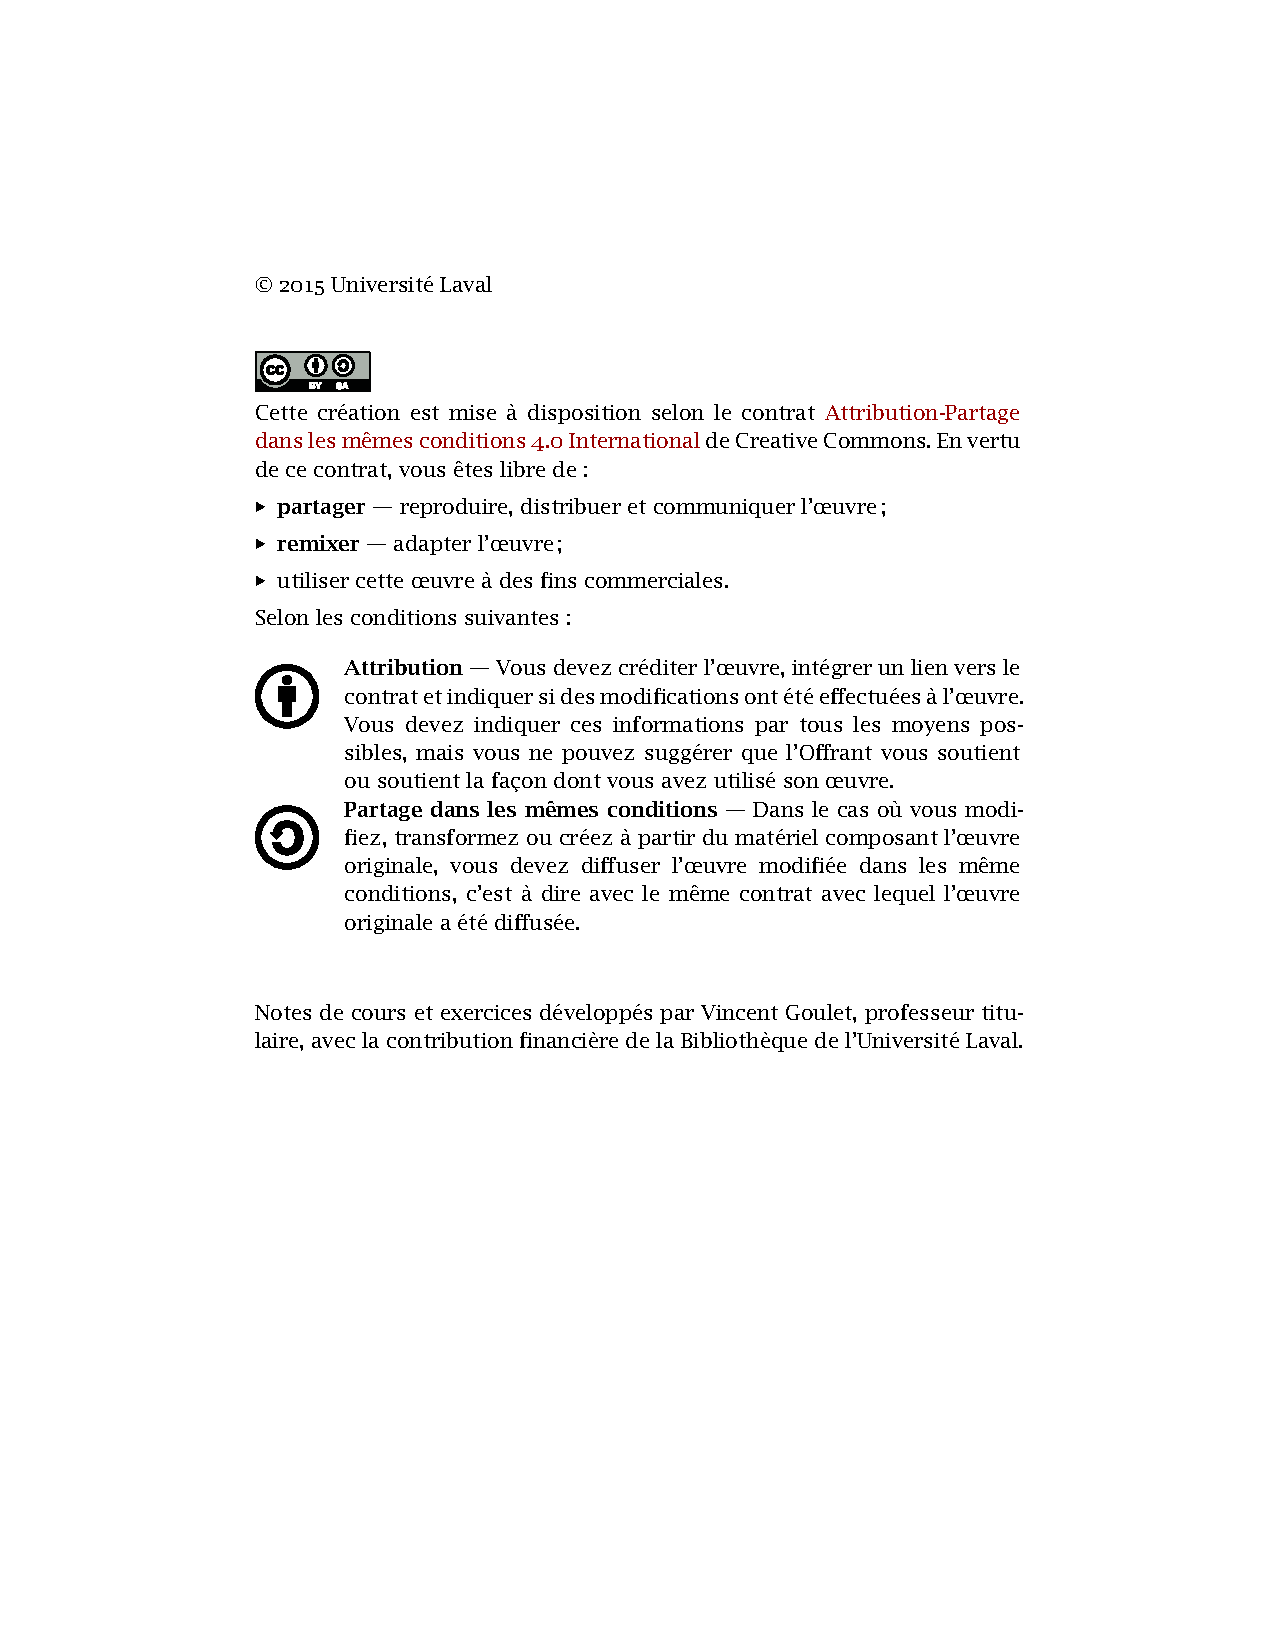
\includepdf[pages=1]{formation_latex-partie_2}
\end{lstlisting}
  \end{sol}
\end{exercice}

\begin{exercice}[nosol]
  Le document \fichier{exercice\_demo.tex} contient plusieurs éléments
  flottants, tableaux et figures. Examiner le code et modifier
  l'argument optionnel de position d'un flottant pour voir son effet
  sur la mise en page du document.
\end{exercice}

\Closesolutionfile{solutions}


%%% Local Variables:
%%% mode: latex
%%% TeX-engine: xetex
%%% TeX-master: "formation_latex-partie_2"
%%% coding: utf-8
%%% End:
